\section{Final System Architecture and Design}

\subsection{System Architecture}
Based on our project's requirements and the components involved, we have decided to use the MVC architecture for our project. We believe that the MVC architecture will best let us integrate the major parts of our project (Web UI, functional logic, and database) effectively. Each are described in more detail down below. 

\subsection{Libraries, Modules \& Packages}
So far, as of sprint 1, we have used tools such as; material UI, bootstrap, Spring Boot, jakarta and deckofcardsapi for our view and our controller and JUnit for model testing.

\subsection{Coding Standards}
\subsubsection{Comments}
Comments (outside of function headers) will always be above the line of code it pertains to, never on the same line. We will aim to keep comments clear, concise and in plain-english.

\subsubsection{Headers}

\begin{itemize}
    \item Function Headers \\
    For functions, we will have consistent headers (in plain-english) including:
    \begin{itemize}
        \item [--] Input: what the function receives as input.
        \item [--] Output: what the function produces.
        \item [--] Purpose: what the function does.
    \end{itemize}

    \item File Headers \\
    For file headers we will have a brief description of what the file is and what it contains.
\end{itemize}

\subsubsection{Variables}
Following the same standard across all of our code, all variables will be camel case and singular. This guarantees consistency in all variable nomenclature. 

\subsubsection{Database}
For our database, our table names will be Pascal case and singular. The primary keys in our database will be camel case followed by 'ID'. The foreign keys will also be camel case with a descriptor followed by 'FK'.\\

Here is an ER diagram of our database: 

\begin{figure}[hbt!]
    \centering
    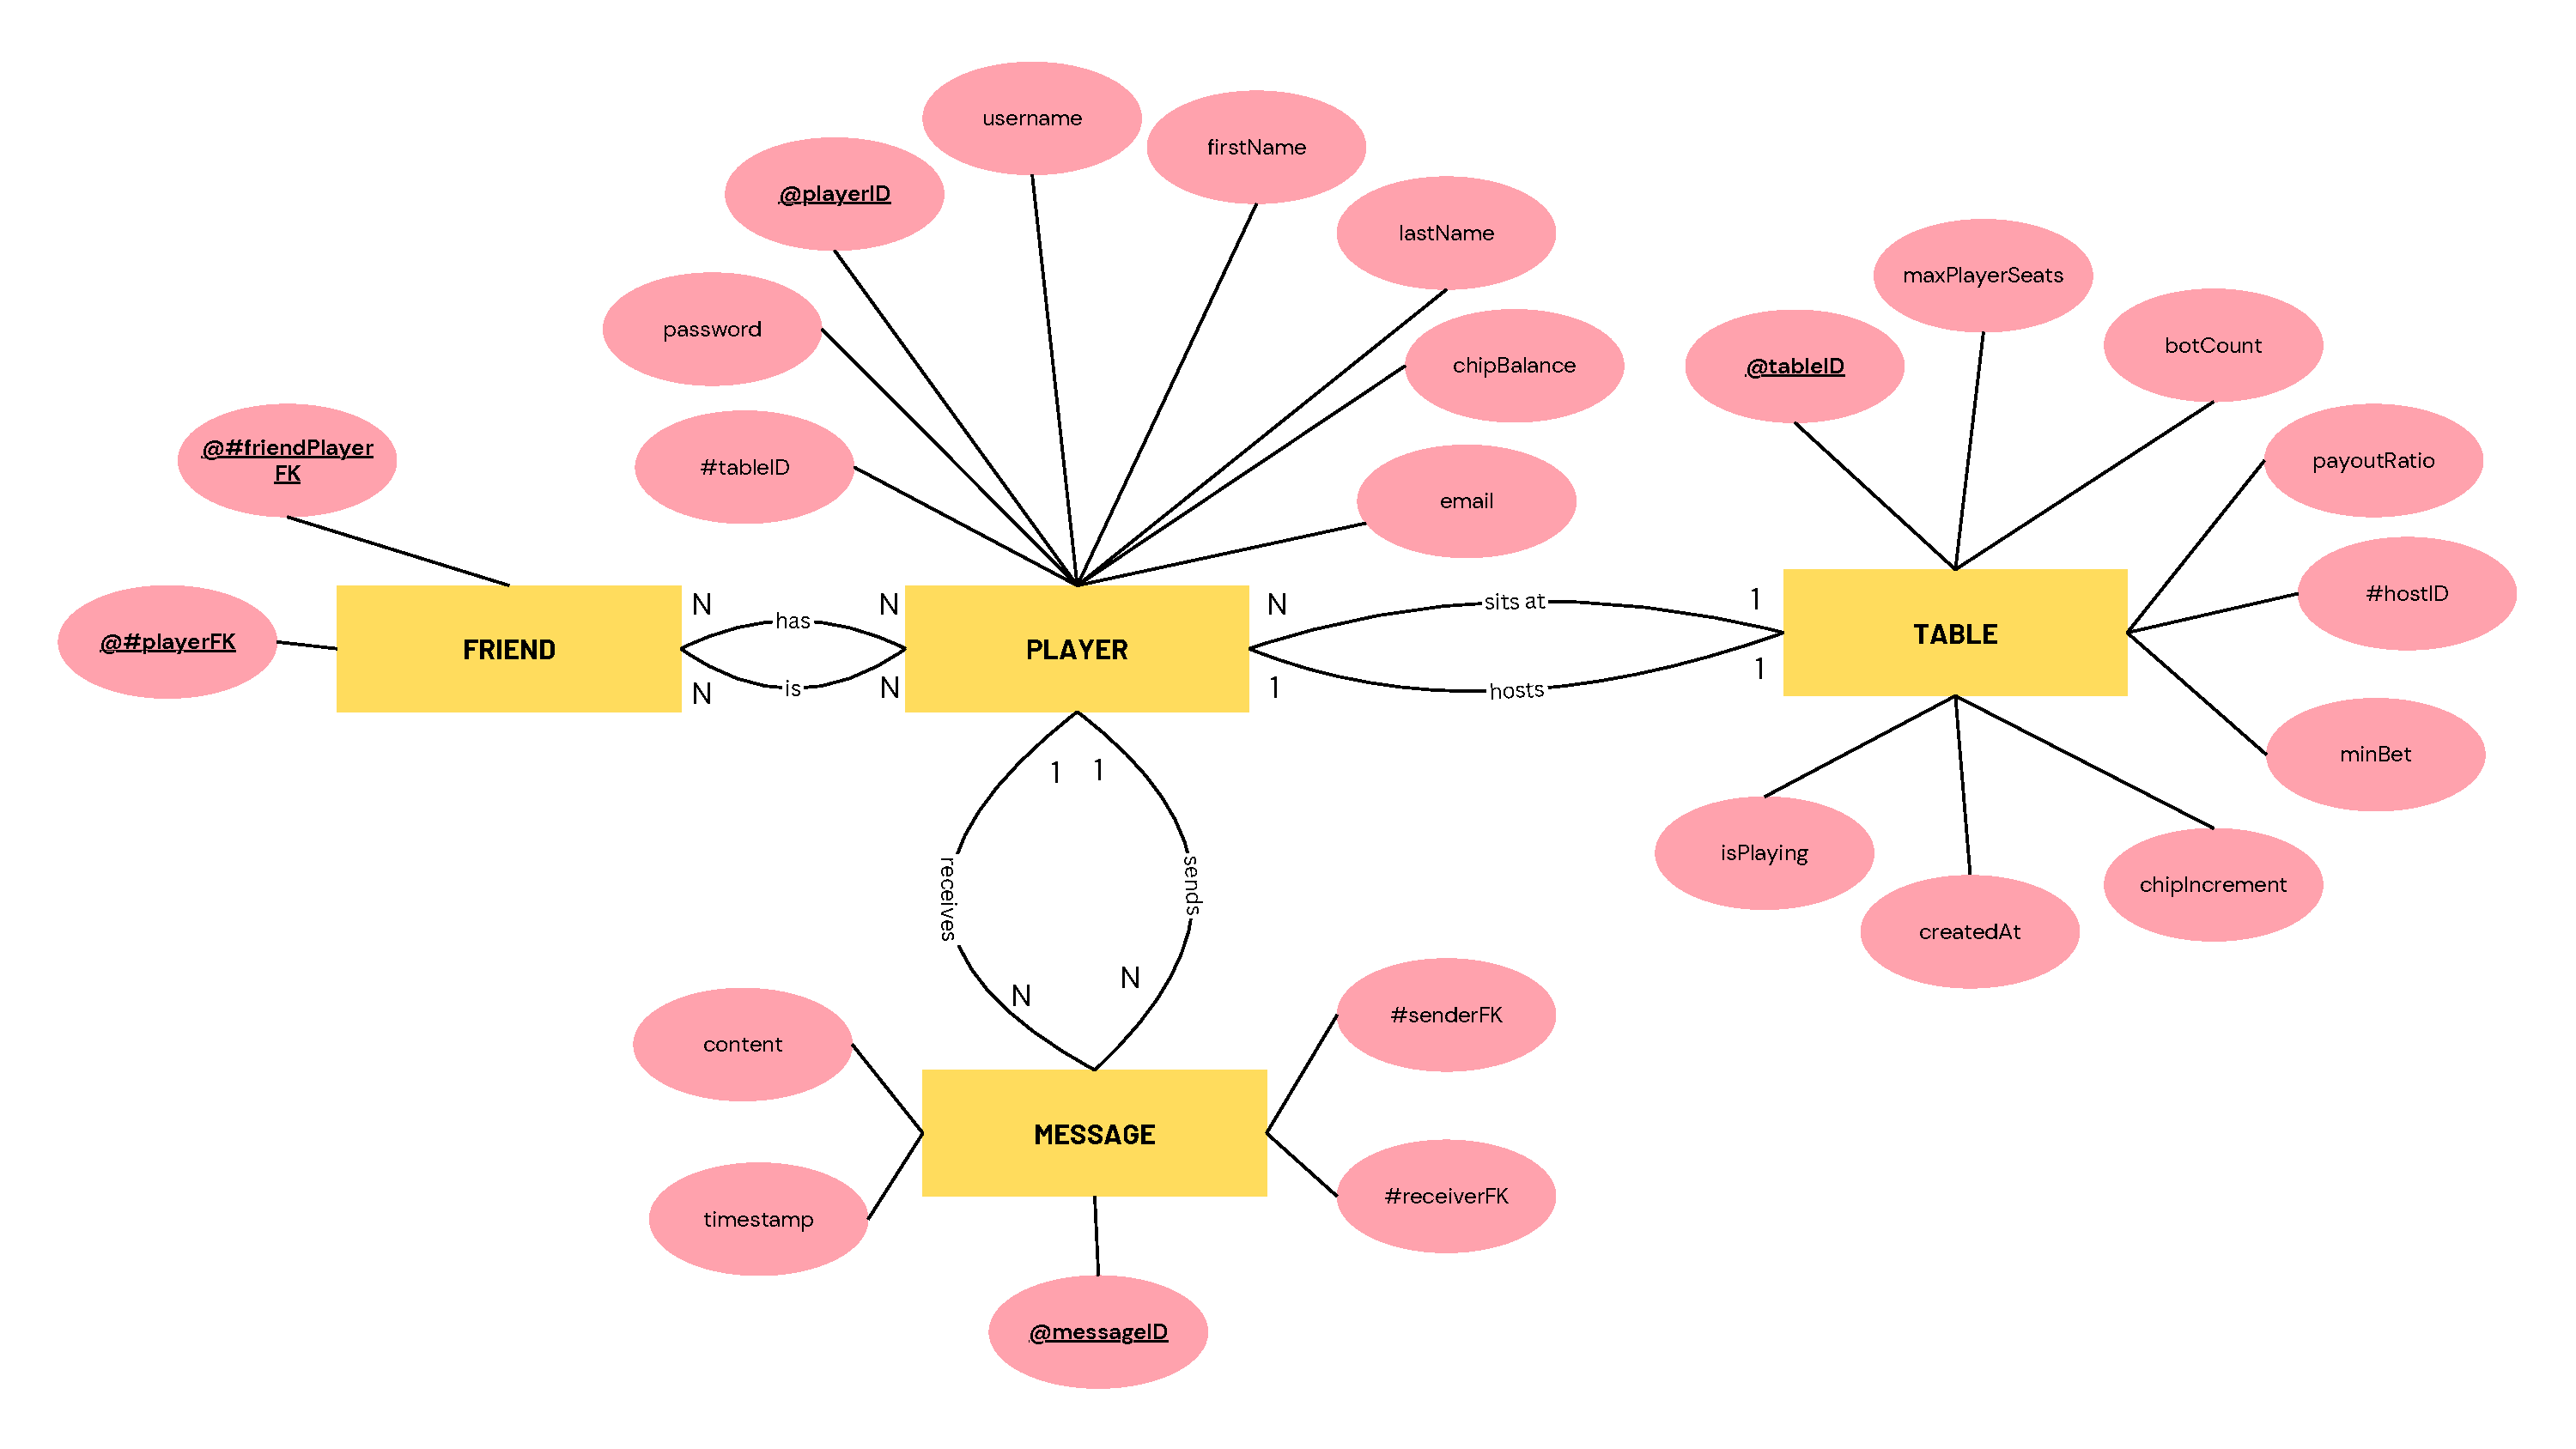
\includegraphics[width=1.0\linewidth]{figures/SE Database ERD.pdf}
    \caption{ERD for our database tables.}
    \label{fig:ERD}
\end{figure} 

\pagebreak

\subsection{Technologies Used}

\subsubsection{Languages}
For the language to run our functional logic we have chose Java as it integrates well with the other languages in our project. For our database components we will be using MySQL along with MySQL community server and MySQL workbench. For our web UI we will be using React along with Next JS for our server.

Here is our UML class diagram that outlines the major classes and relations in our software:  

\begin{figure}[hbt!]
    \centering
    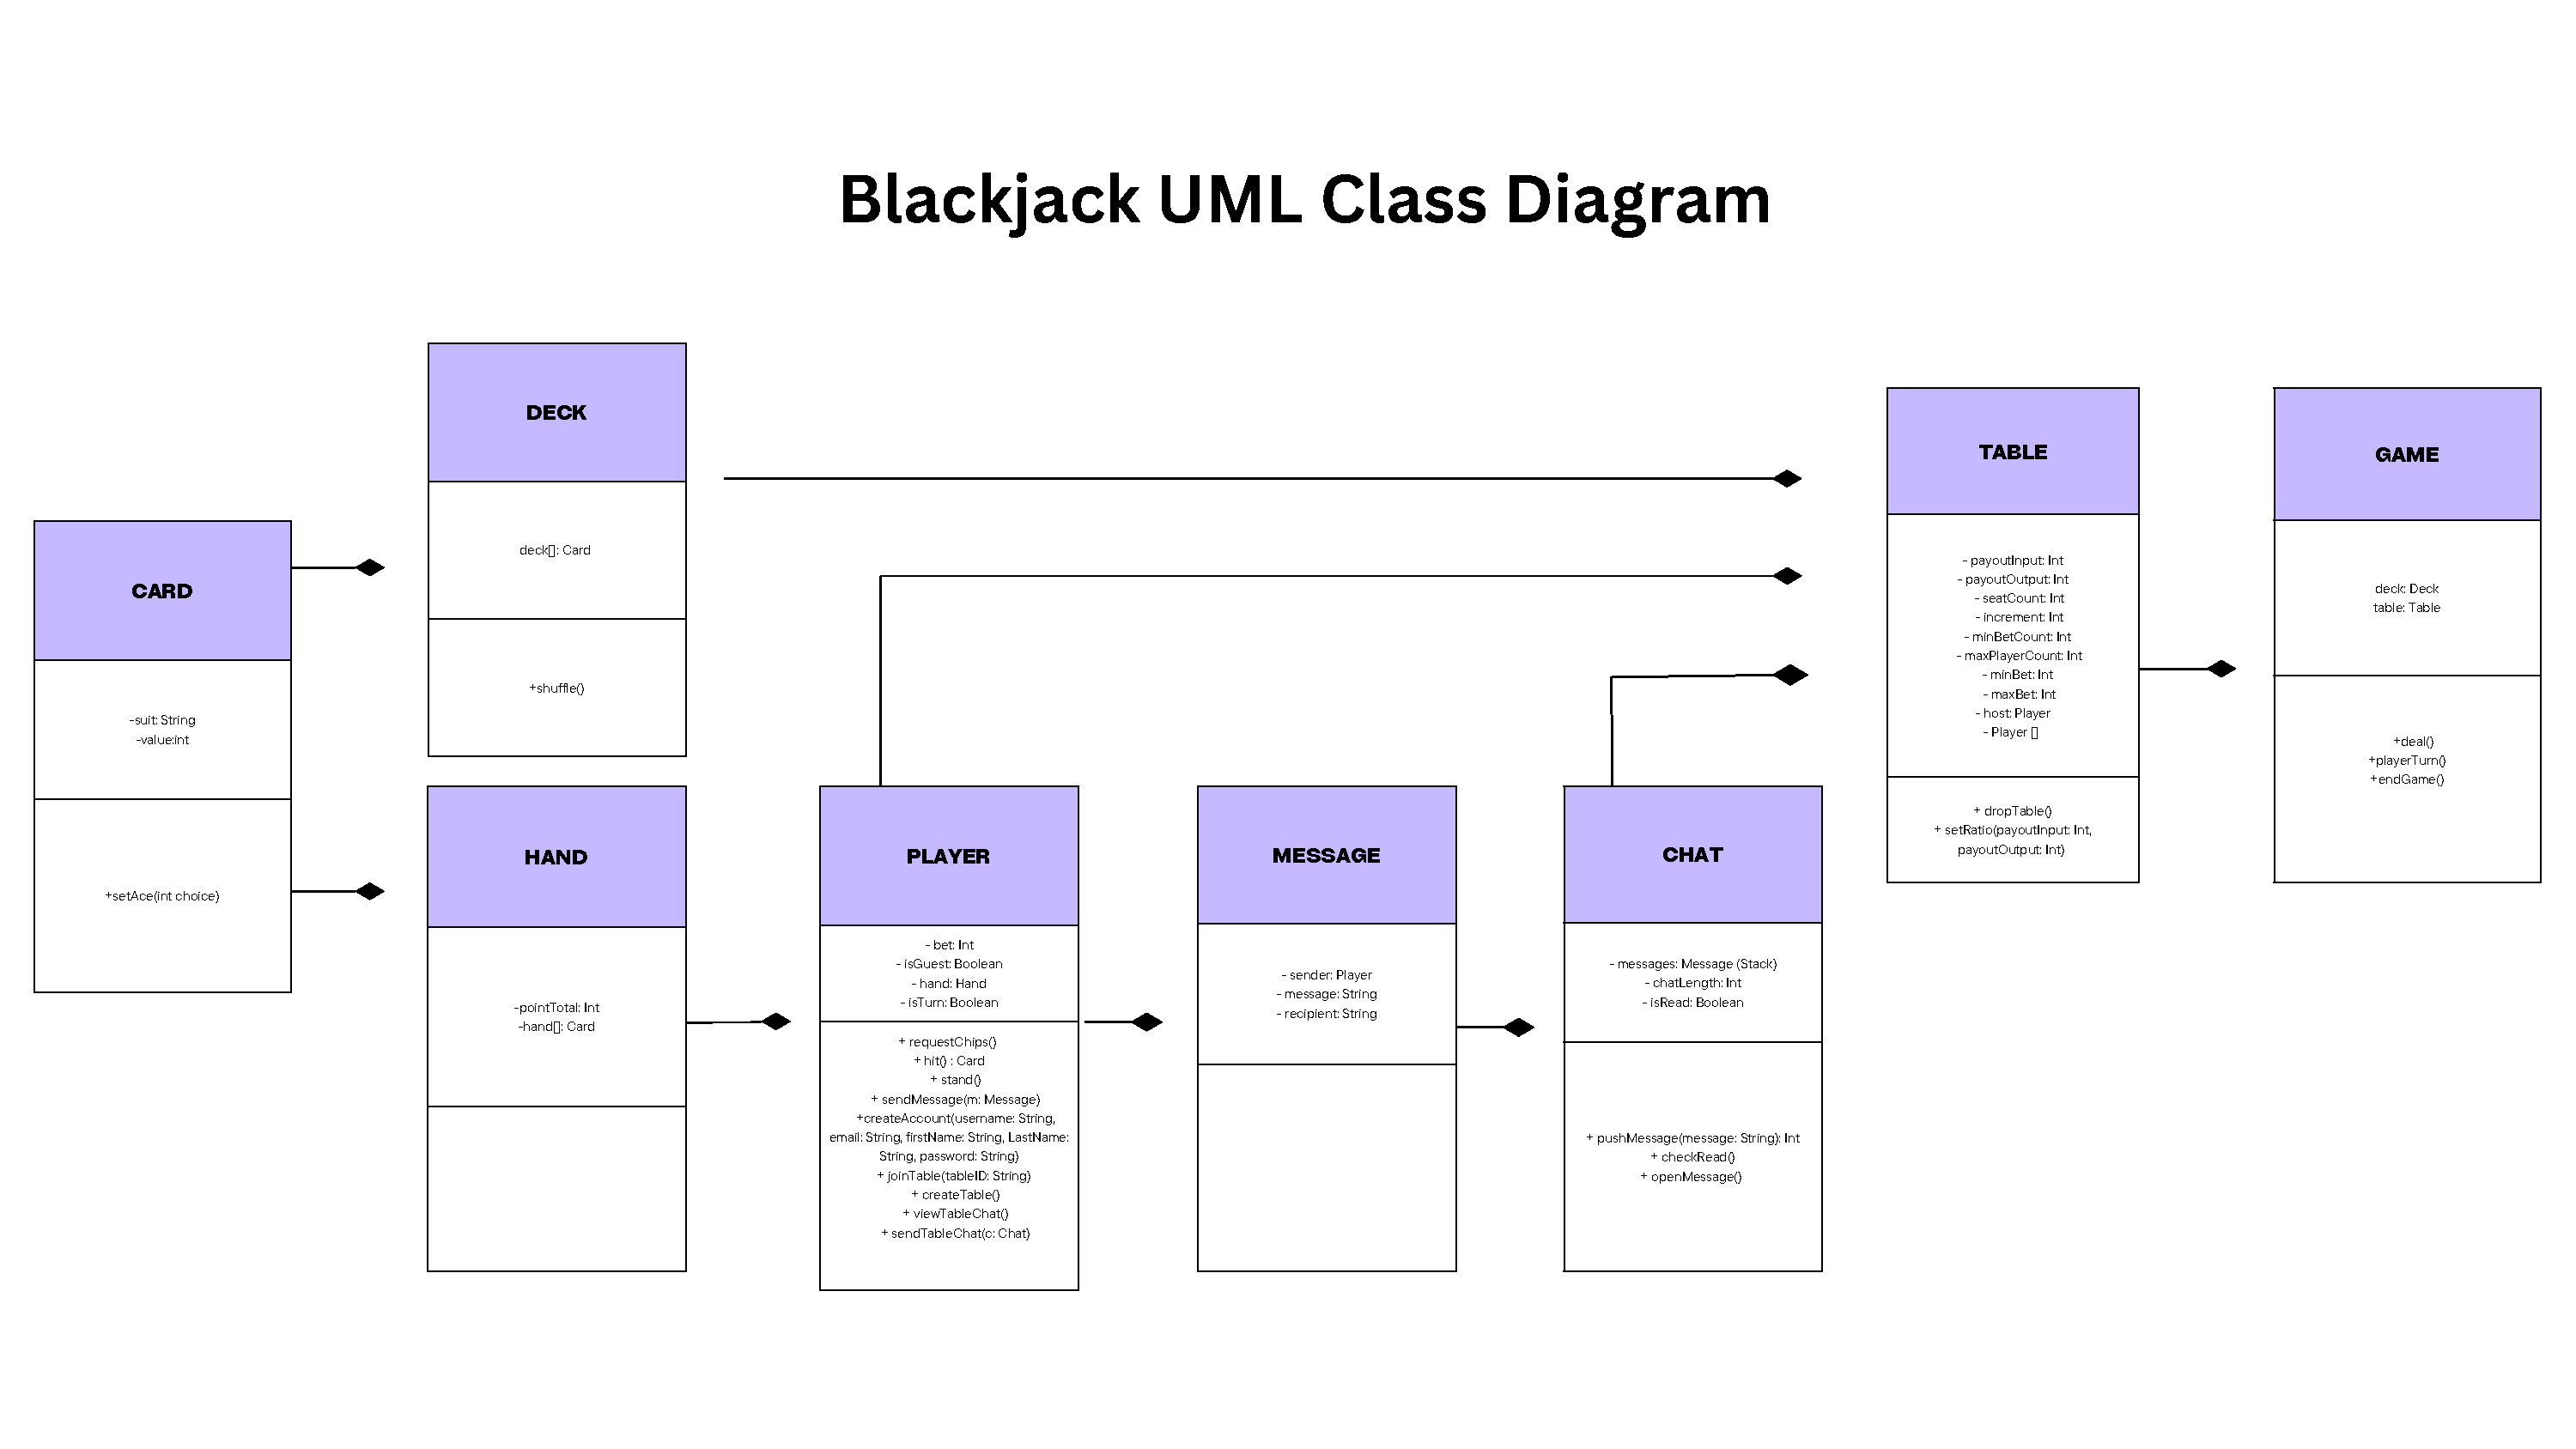
\includegraphics[width=0.8\linewidth]{figures/UML Diagram Whiteboard.pdf}
    \caption{UML diagram of major classes and relations.}
    \label{fig:UML}
\end{figure}

\pagebreak

\subsection{UI Mockups}
Here are some of the initial UI designs for our project:

\begin{figure}[hbt!]
    \centering
    
\includegraphics[width=0.5\textwidth]{figures/Blackjack.png} \\
    \caption{This is the UI mockup for the logo of the app (illus. Emma Heiser)}
    \label{fig:logo}
\end{figure}

\begin{figure}[hbt!]
    \centering
    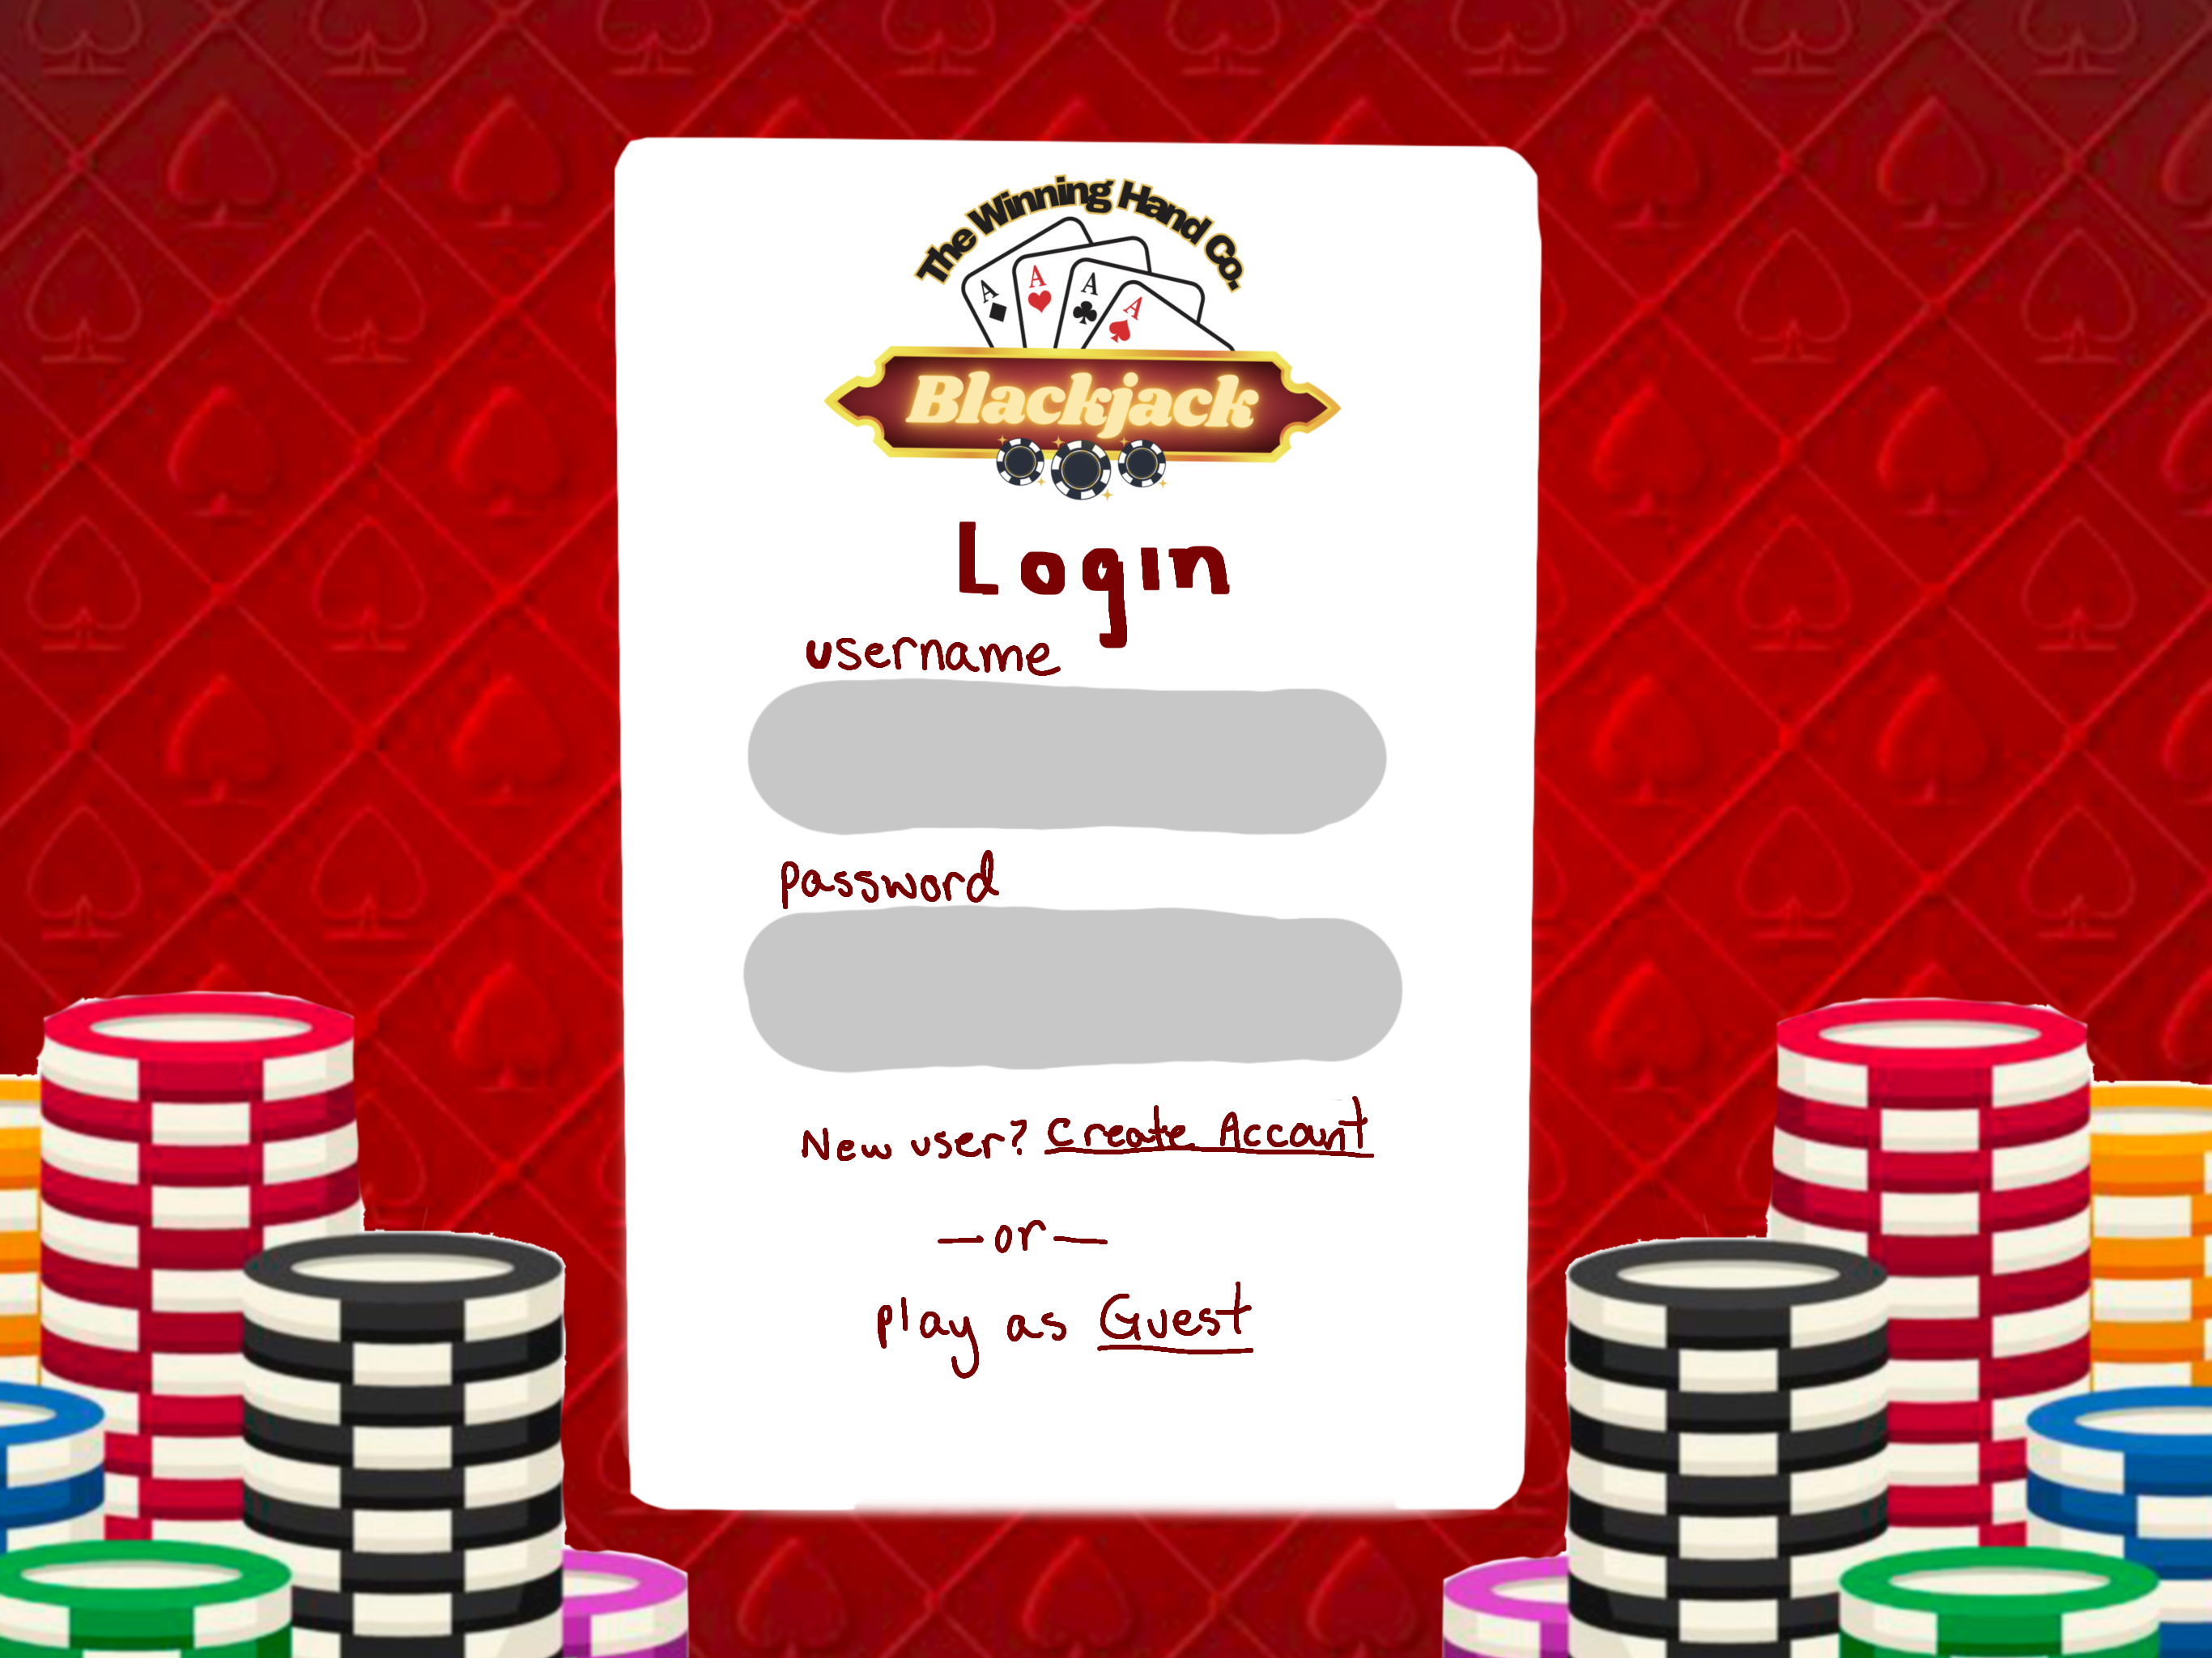
\includegraphics[width=0.75\linewidth]{figures/login.png}
    \caption{This is a UI mockup of the login screen (illus. Emma Heiser)}
    \label{fig:login}
\end{figure}

\begin{figure}[hbt!]
    \centering
    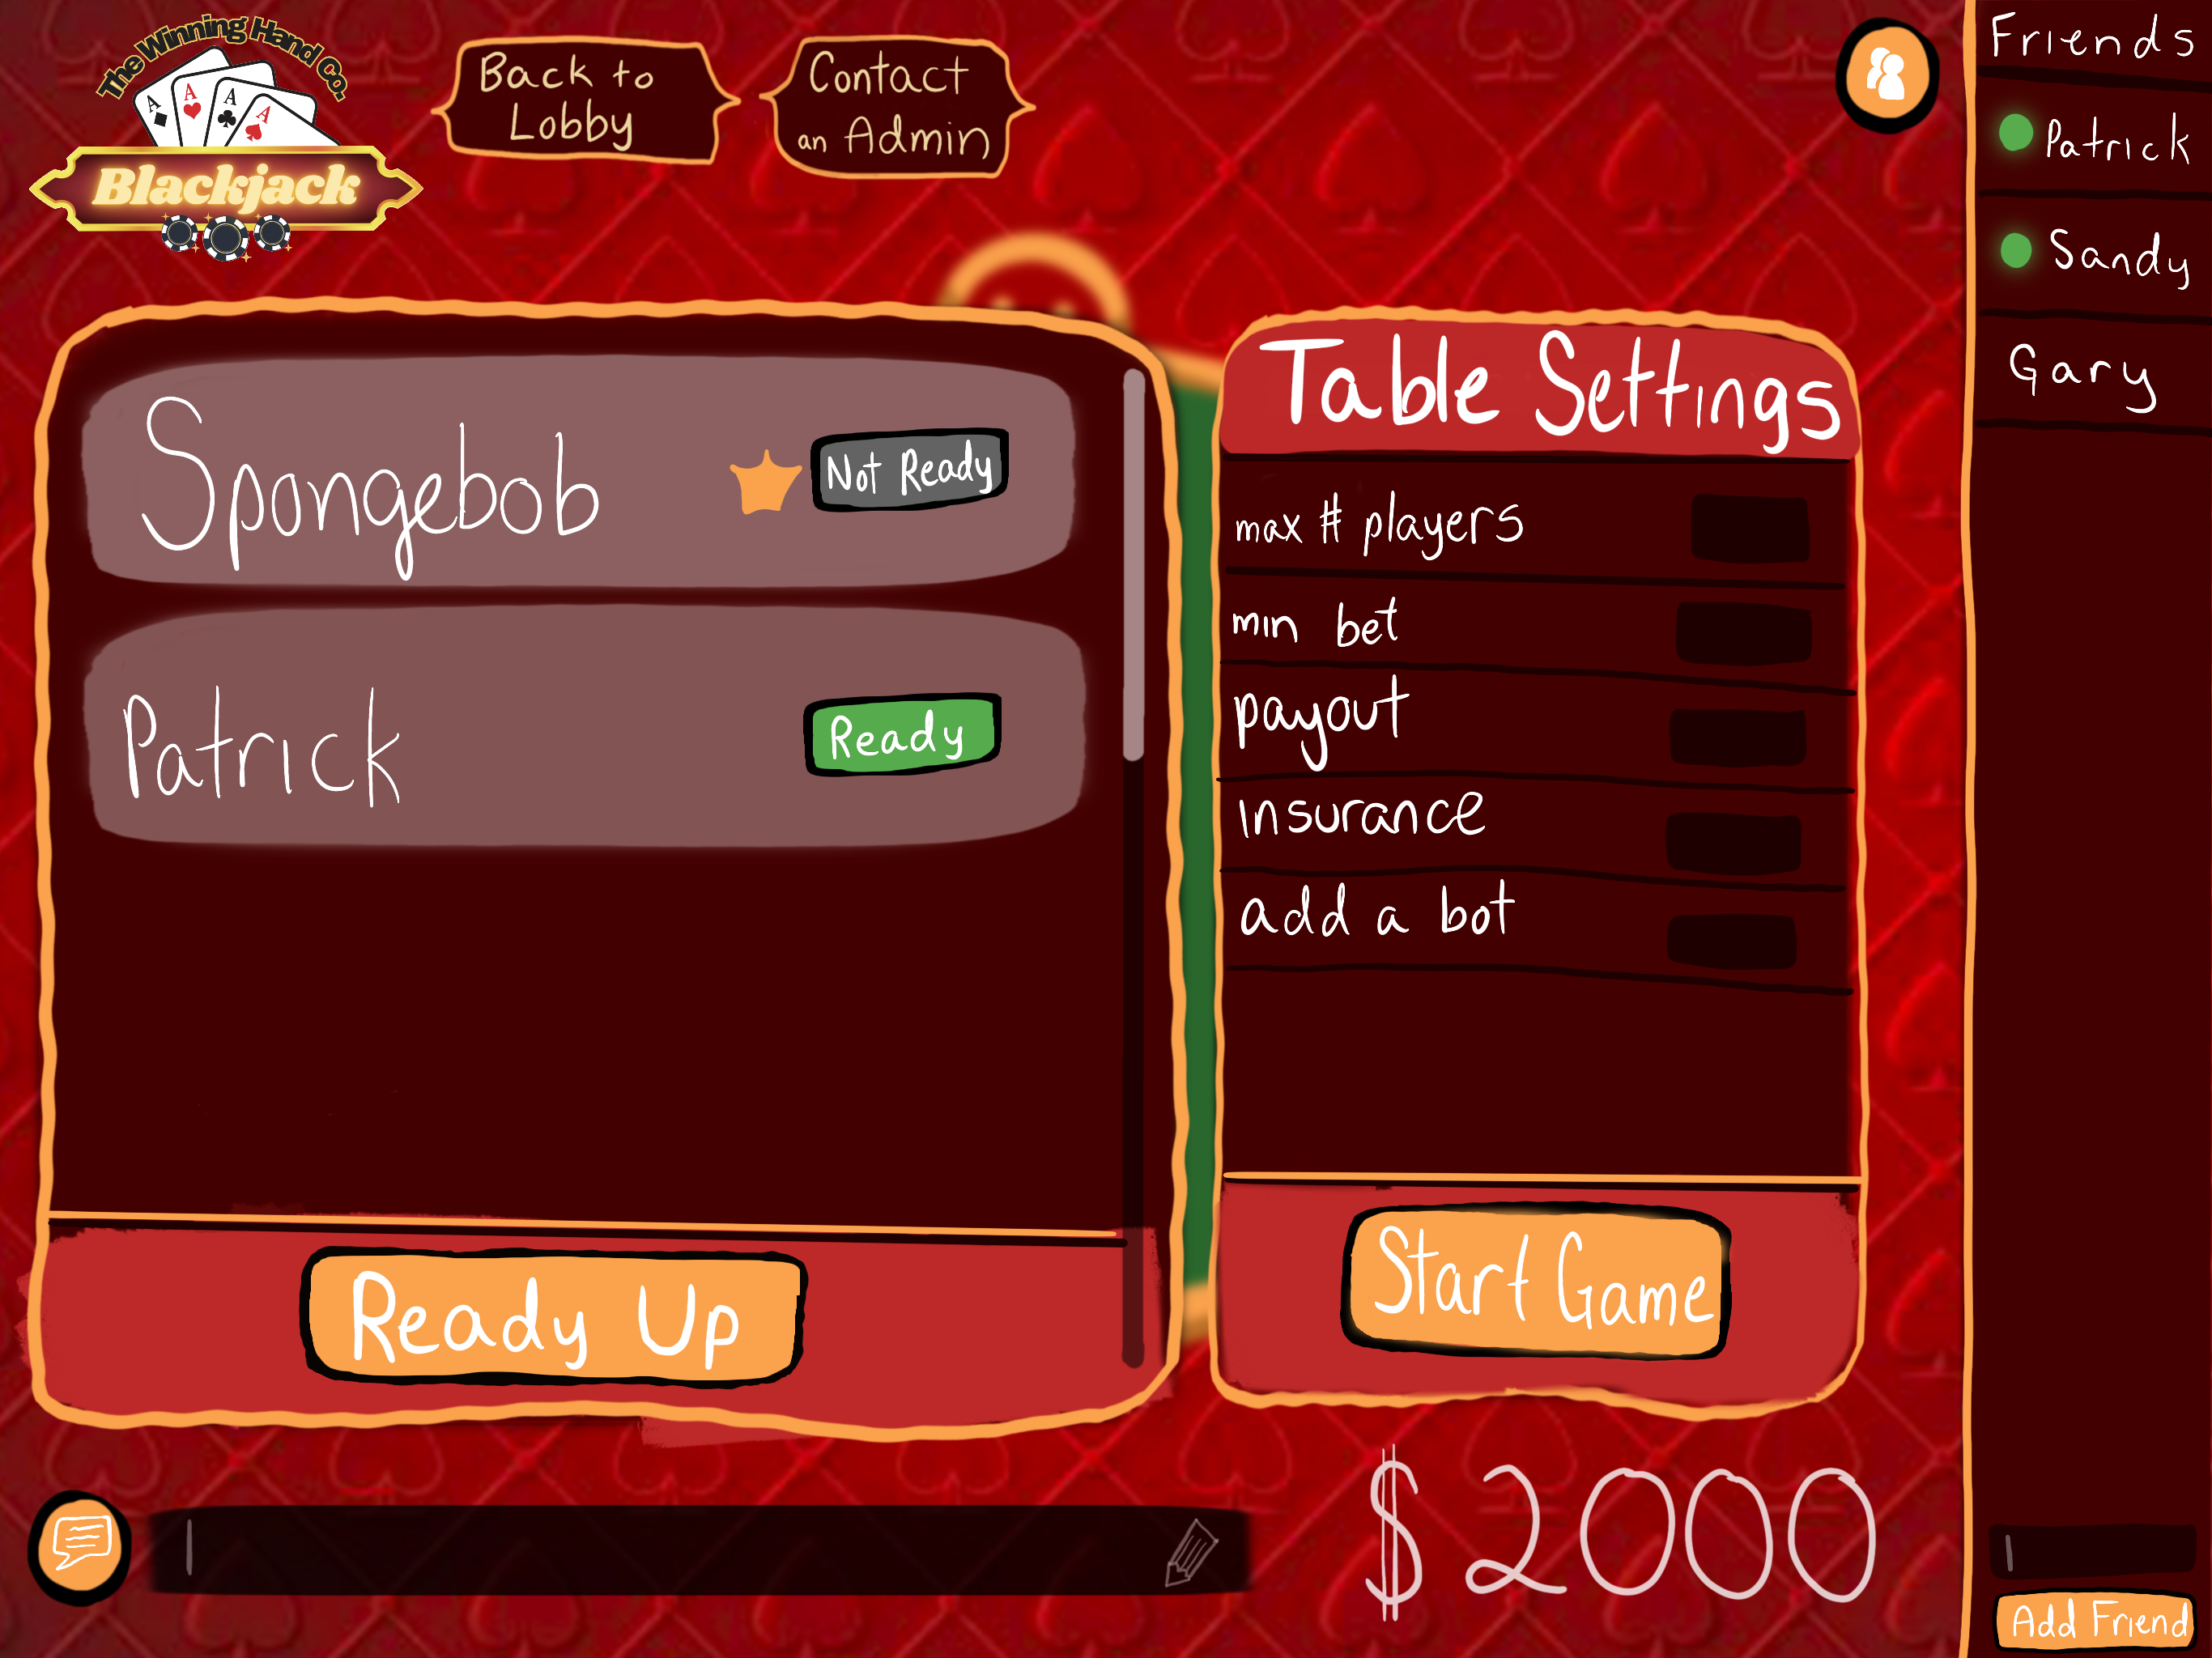
\includegraphics[width=0.75\linewidth]{figures/at-table.png}
    \caption{This is the UI mockup of creating a table (illus. Emma Heiser)}
    \label{fig:table}
\end{figure}

\pagebreak

\begin{figure}[hbt!]
    \centering
    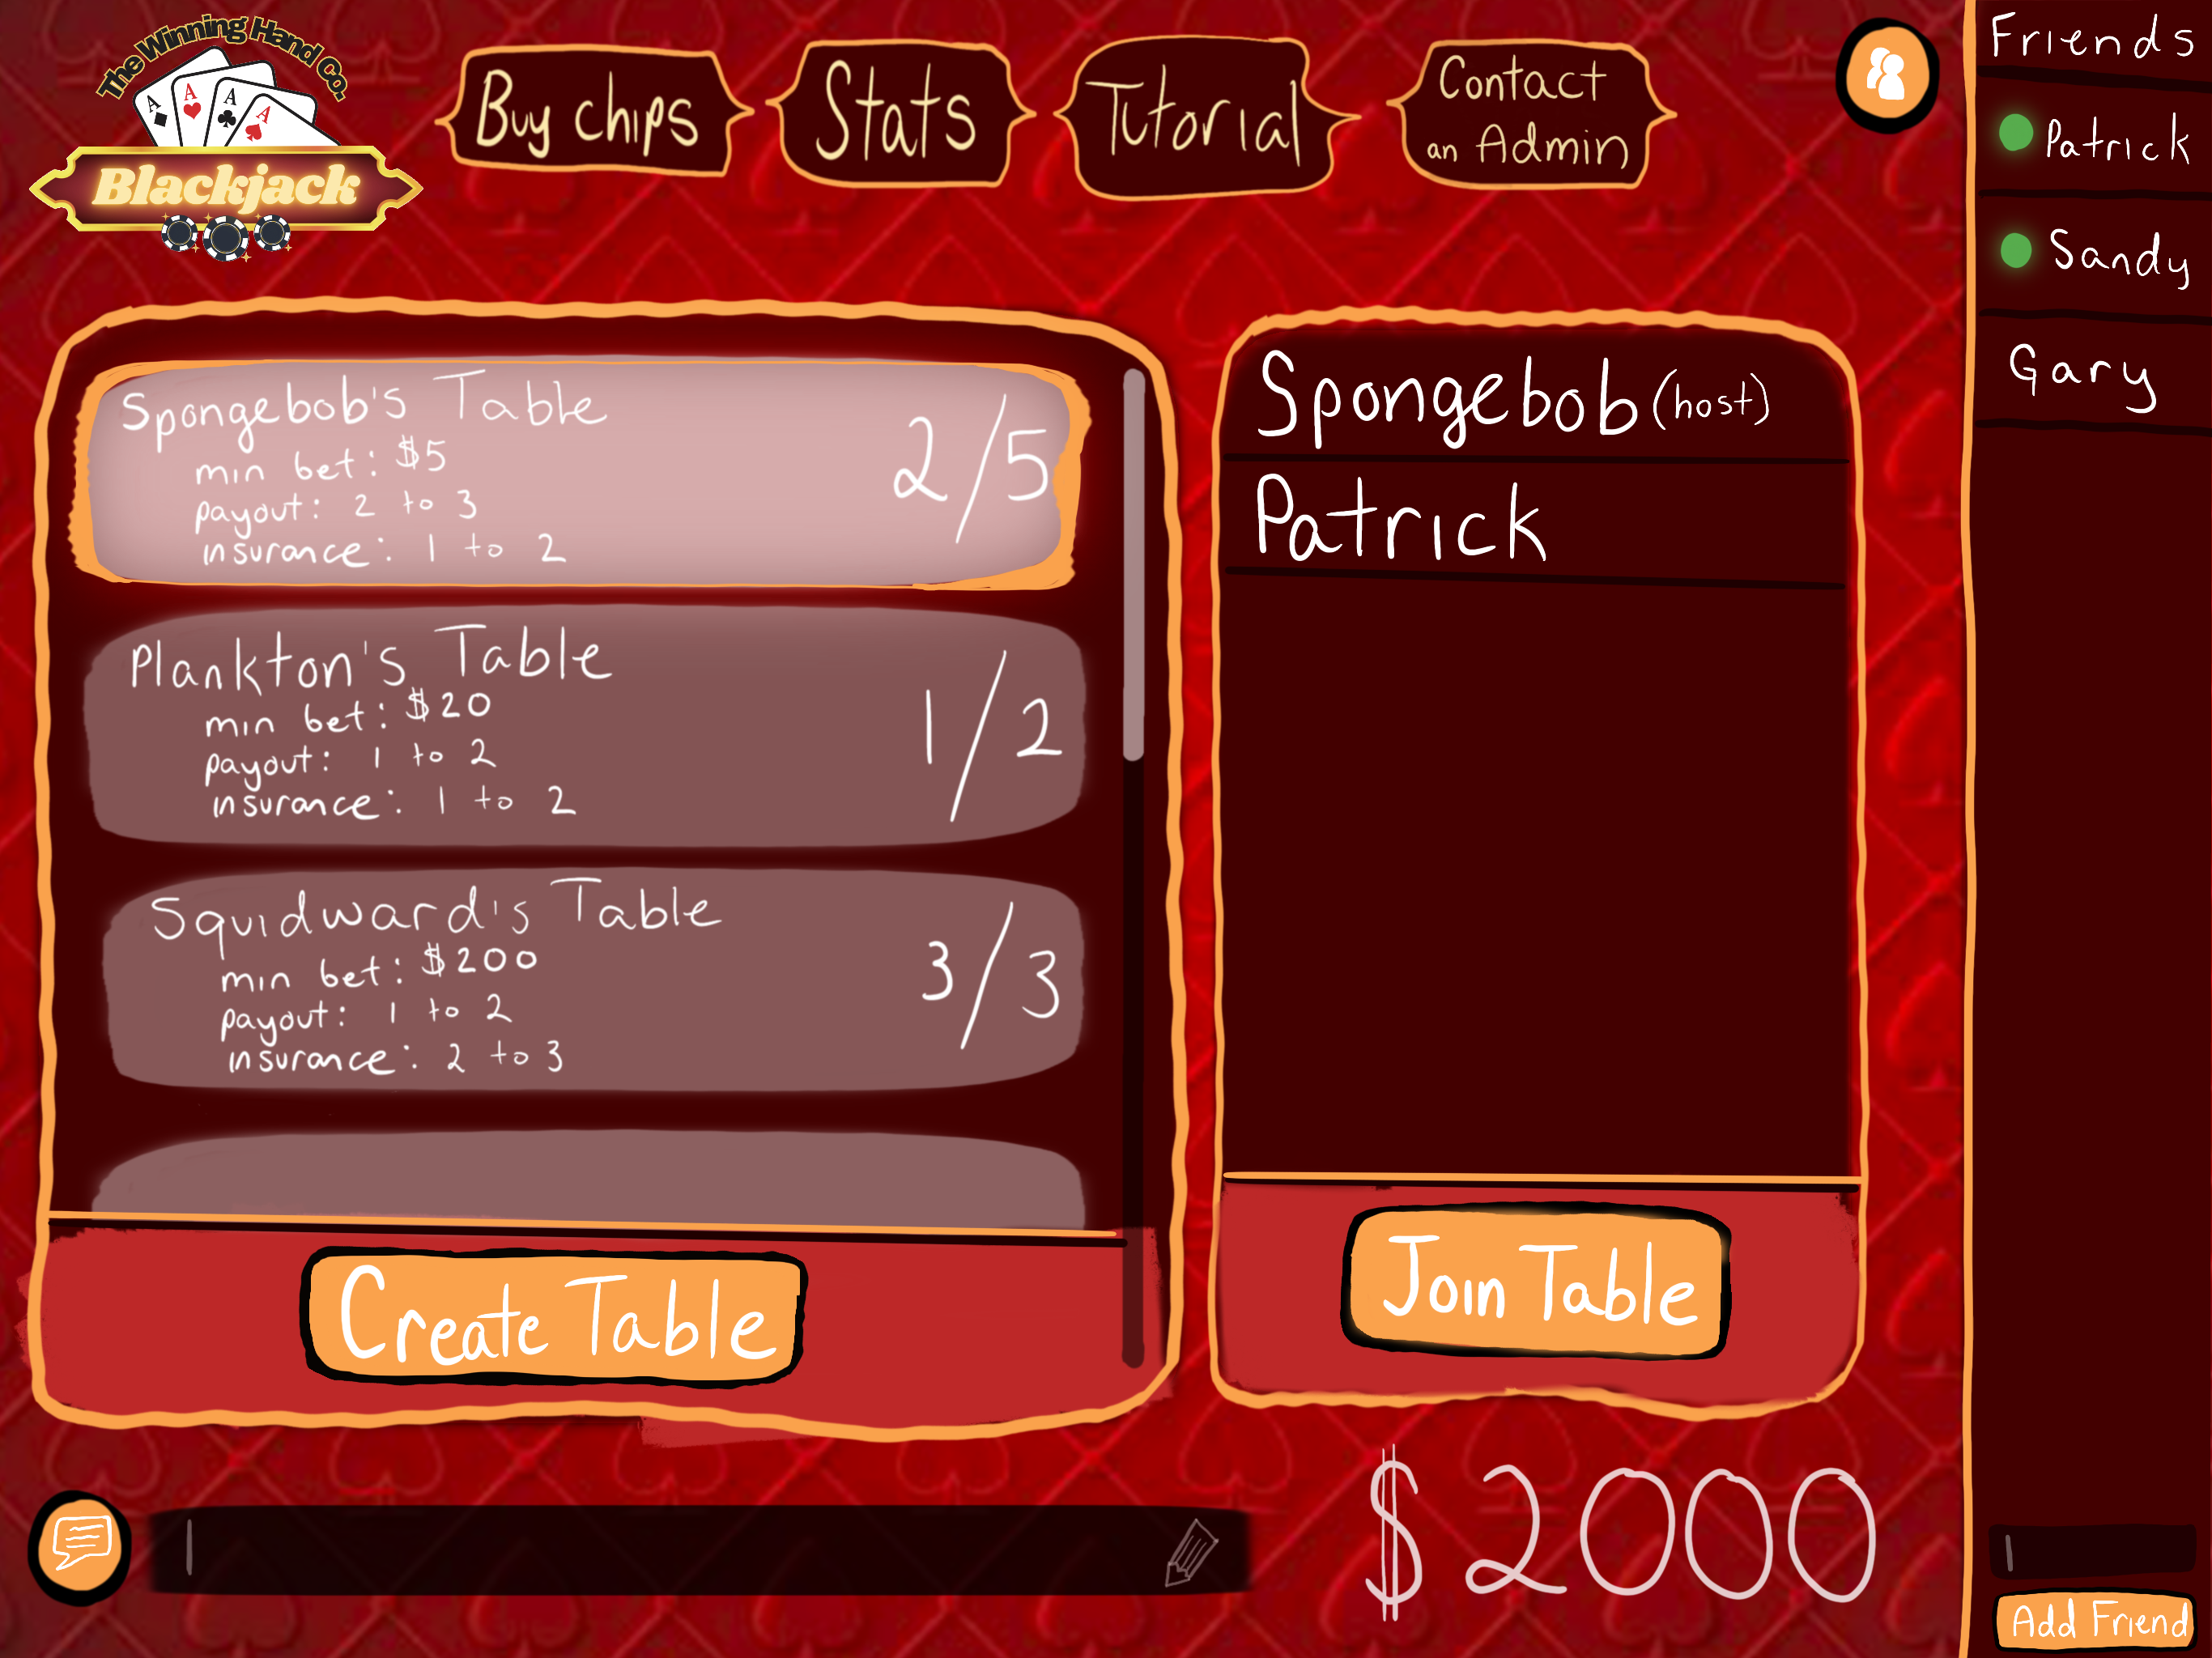
\includegraphics[width=0.75\linewidth]{figures/lobby.png}
    \caption{This is the UI mockup for the lobby where players can see available tables (illus. Emma Heiser)}
    \label{fig:lobby}
\end{figure}

\begin{figure}[hbt!]
    \centering
    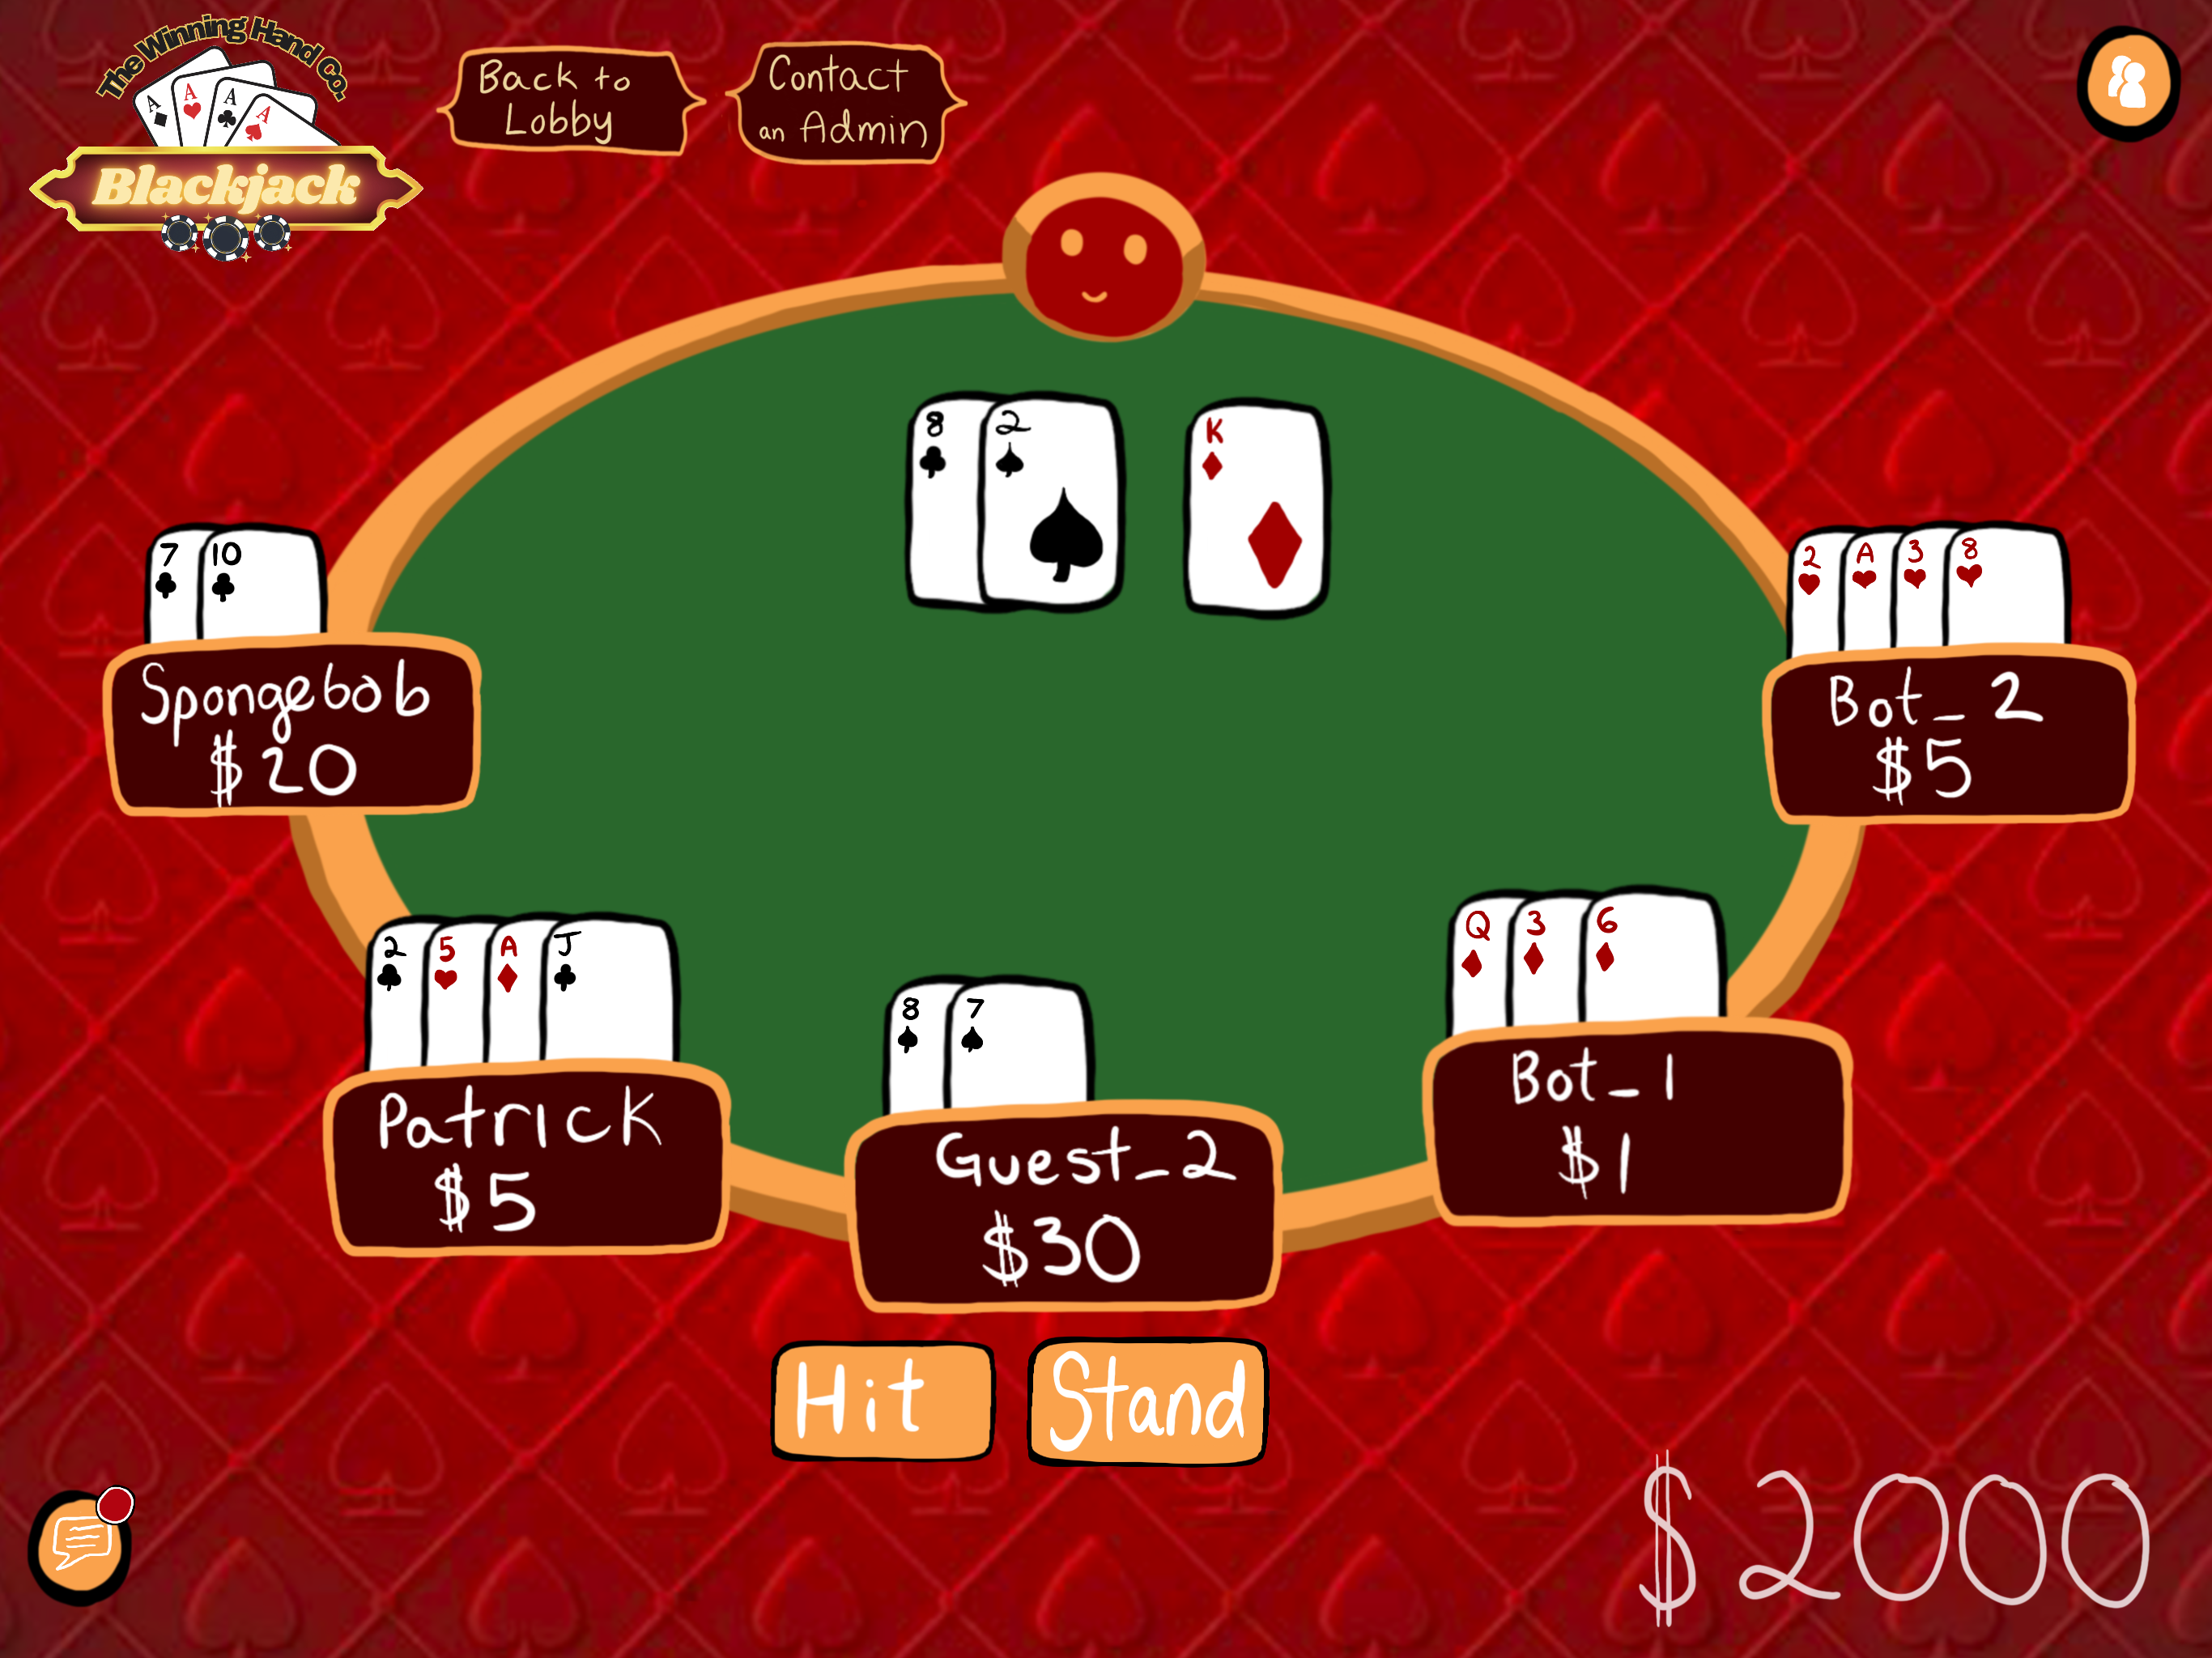
\includegraphics[width=0.75\linewidth]{figures/in-game.png}
    \caption{This is the UI mockup of the game being played at a table (illus. Emma Heiser)}
    \label{fig:game}
\end{figure}

\pagebreak
